\documentclass[12pt,letterpaper]{article}

%%%%%%%%%%%%%%%%%%%%%%%%%%%%%%%%%%%%%%%%%%%%%%%%%%%%%%%%%%%%%%%%%%%%%%%%%
\pagestyle{plain}                                                      %%
%%%%%%%%%% EXACT 1in MARGINS %%%%%%%                                   %%
\setlength{\textwidth}{6.5in}     %%                                   %%
\setlength{\oddsidemargin}{0in}   %% (It is recommended that you       %%
\setlength{\evensidemargin}{0in}  %%  not change these parameters,     %%
\setlength{\textheight}{8.8in}    %%  at the risk of having your       %%
\setlength{\topmargin}{0in}       %%  proposal dismissed on the basis  %%
\setlength{\headheight}{0in}      %%  of incorrect formatting!!!)      %%
\setlength{\headsep}{0in}         %%                                   %%
\setlength{\footskip}{0.2in}       %%                                  %%
%%%%%%%%%%%%%%%%%%%%%%%%%%%%%%%%%%%%                                   %%
\newcommand{\required}[1]{\section*{\hfill #1 \hfill}}               %%
\renewcommand{\refname}{\hfill References Cited \hfill}                %%
\bibliographystyle{abbrv}                                              %%
%%%%%%%%%%%%%%%%%%%%%%%%%%%%%%%%%%%%%%%%%%%%%%%%%%%%%%%%%%%%%%%%%%%%%%%%%


\usepackage{mathptmx}
\usepackage{graphicx}
\usepackage{url}
\usepackage[bookmarks=false]{hyperref}
\usepackage{subfig}
\usepackage{wrapfig}

\usepackage{stfloats}
\usepackage{paralist}
\usepackage{aas_macros}

%%% These are just for removing vertical spaces
\usepackage{mdwlist}
\usepackage[medium,compact]{titlesec}
\titlespacing{\section}{0pt}{*0}{*0}
\titlespacing{\subsection}{0pt}{*0}{*0}
\titlespacing{\subsubsection}{0pt}{*0}{*0}

\setlength{\parskip}{0.3em}
\setlength{\parsep}{0em}
\setlength{\headsep}{0em}
\setlength{\partopsep}{0em} 
\setlength{\parindent}{0em} 

\addtolength{\floatsep}{-1em}
\addtolength{\textfloatsep}{-1em}
\addtolength{\abovecaptionskip}{-0.5em}
%%%

\newcommand{\etal}{~\emph{et~al.}~}

\begin{document}

\required{Unleashing ALMA for Big Data}

\section{Summary}

This is the final report for the ALMA Development Study on enhancing
user access to the science data in large ALMA data cubes and
creating an environment for scientific data mining. The top
goal of this study was to create a well-defined plan for
development of the software infrastructure and prototype 
key applications for enabling science with large image cubes.
The second goal was to scope the manpower and cost for achieving
a specific level of functionality which brings strong scientific
value. Based on the work done in this study, this team wrote
an ALMA Development Project Proposal to implement an XML 
infrastructure and tool set. The costs and man-power requirements
are presented in the proposal and are not reported here.

The main body of this report presents study results in the
five proposed areas. First area: in access performance, we found
that speed of access to data in CASA image format was efficient
if the data were being accessed in the optimal sequence for the
tiling; it can be inefficient if accessed against the ``grain''
of the tiling. This feature of tiling can be minimized by taking
advantage of larger memory capacities in new generations of machines
and allowing for a few different tiling choices where appropriate.

Second area: we developed a set of goals for our proposed tool set
and a technical approach for our package which we call ADMIT:
ALMA Data MIning Toolkit. We present a conceptual overview of the
design and operation and how ADMIT fits into the ALMA and CASA
environment.

Third area: we prototyped some tools for ADMIT as examples of what
can be done and as mechanisms for defining the way that ADMIT infrastructure
and tools can interact.

Fourth area: we explored a number of new algorithms that would enhance
user ability to understand the science content of large data cubes. 
We specifically discuss the overlap integral and descriptor vectors.

Fifth area: the interface between modeling and simulation data and
observational data de-emphasized as a study area so that more time
could be spend in areas two, three, and four, and the Conceptual
Design Document

The first accompanying memo summaries the results of timing measurements
of access to data by a number different programs for a number of
different data configurations. 

The second accompanying memo is a Conceptual Design Document for ADMIT.


\clearpage \setcounter{page}{1}

\section{Introduction}

ALMA will enable groundbreaking science over a wide range of fields. 
Exciting discoveries will be made with simple images of continuum 
emission and/or individual molecular lines. For many areas of science, 
however, such images are the tip of the iceberg; large multi-channel
data cubes and large area maps will exploit the greater capability
of ALMA.  ALMA's high sensitivity and large correlator enable
the collection of large spectral data cubes which contain a wealth of
information about the kinematic, physical, and chemical state of the 
galaxies, molecular clouds, circumstellar disks, and evolved stars under study. 
ALMA's speed can enable wide field mappings and large sample surveys.
The overall goal of this study is to outline
the tools for effectively deriving science from
large ALMA data cubes. We seek to facilitate standard 
scientific analysis and to enable new and creative ways to derive 
science from the cubes.  

The original focus areas in the study as stated in the first
section of the proposal were:
\begin{itemize}
\item ``interfaces to CASA image cubes and infrastructure for efficient, versatile access to 
these cubes in an open-source/application environment;
\item design of metadata structures that would accompany the astronomical and image data 
to enhance the utility of applications;
\item options for quantitative visualization and the speed/capability trade-offs;
\item applicability of and development paths for existing algorithms in the computer 
science community to identify and quantify structure of astronomical interest in large data cubes.
\item interfaces for intercomparison of computational models with observational data ''
\end{itemize}

These focus areas were refined over the course of the study. 
For example, the visualization area was de-emphasized in our study because 
a selected 2012 ALMA Development Study lead by Eric Rosolowsky focused
on visualization of ALMA datasets. One of our team members (Peter Teuben)
became an outside collaborator on that team; this facilitated information
exchange and reduced overlapping efforts. Second,
as a part of the study effort, we came to realize that the file size, 
Internet transfer time, and complexity of the data cubes (multiple windows
with many channels) were themselves impediments for typical users trying to 
access the science in their data. These complexities represent an even
larger barrier for scientists new to the radio field. Hence we expanded
our study in this direction.

The following sections summarize the activities and outcomes of the study
organized into sections following the above five itemized study areas.
The two appended documents provide: (A) discussion of the problem of optimizing
speed of computer access to the data and (B) an conceptual design document 
for an ``ALMA Data Mining Tool (ADMIT)''.  

This study established the groundwork for a proposal for ADMIT
that was submitted for the 2013 ALMA Call for Development Projects.




\section{Access to CASA Image Cubes}

We started our study by looking at approaches for accessing large
ALMA datasets. Since image cubes, not {\it u,v} data, are the
focus of this study, we looked at the access speeds for various
operations to data cubes in a number of different formats including
the CASA tiled data format. Not too surprisingly, tiled data
access works very well for balanced cubes, but slower 
access in some of the directions for stick-like cubes (large in the
z-dimension compared to x and y).
This is detailed in the attached memo.

In the course of this work, and from discussions with CASA programmers,
several points were clear. First, CASA made the decision to follow a
tiled storage approach rather than a memory intensive model. CASA has
been effective in implementing this strategy.
With the expanding capabilities of machines and
the decrease in memory cost, it is attractive to consider tuning CASA
to be more memory based.
The tiled data storage approach of CASA is
efficient when the data are being accessed in a sequence which
follows the tiling; it can be significantly less efficient
for access which is against the grain of the tiling scheme. 
While the tile definition can be tuned to the expected access pattern
to give better performance, this is not currently utilized in CASA
as an active option.

{\it Recommendations: CASA should periodically review the memory model
for the prototype user machine and tune CASA image storage as possible to optimize
memory usage. CASA should review the usage patterns of programs to
optimized the tiling for the most commonly used programs. There may be
circumstances where it is sufficiently compute efficient to encourage users
to store a given dataset in multiple tiling formats.}

Given the evolving capability of machines and CASA, it was clear to us
that there was no strong advantage to another data storage format to increase
general compute speed at the cost additional disk usage. This conclusion
might have been different if we had been focused on a specific visualization
tool or application.



\section{Science Metadata and the User}

It became very clear to us while
working with public access ALMA Cycle 0 data that efficient
access was about more than just compute efficiency. Current
ALMA datasets are contained in multiple large tar files which
can be very costly in time to download. The cubes for each band
have a large number of channels without information about what
lines are in what channels. It is not a simple and efficient
interface for the user of the science content in the data.

A large fraction of our study focused on the design of an
XML-based scientific meta-data system and the design of
tools that can be build on that system.

The concept is to create a value-added software package that integrates with the ALMA 
archive and CASA to provide scientists with immediate access to traditional science 
data products such as moment maps, and provide innovative tools for exploring data cubes. 
The proposed package is called ADMIT, for ALMA Data Mining Toolkit, a software suite 
that creates value-added data products from ALMA data image cubes directly from the 
ALMA pipeline for ingestion into the archive and provides a standalone 
infrastructure and applications for mining user-downloaded cubes. 

The top-line goals of the ADMIT are to: 

\begin{itemize}
\item[] (1) make the scientific value of ALMA data more immediate to all users, 
\item[] (2) create an analysis infrastructure that allows users to build new tools,
\item[] (3) provide new types of tools for mining the science in ALMA data, and
\item[] (4) increase the scientific value of the rich data archive that ALMA is creating.
\end{itemize}

ADMIT would provide capabilities, missing in the current ALMA baseline system, 
that are key to achieving ALMA’s full science potential for both proposers and archival data users.  
The following are the top-line goals for the system and how they can be achieved:

\noindent
{\bf Goal 1: To provide an immediate data access capability.}  This will be accomplished by 
creating a set of basic data products (BDP) which are included into the archive and 
available to the users for quick overviews of their data. The BDP are a combination of 
XML files, PNG images, and FITS files that will be produced by ADMIT software 
(a combination of Python scripts and CASA programs) from the ALMA approved pipeline 
image cubes (all correlator bands). The BDP consist of harvested header information 
about the source and observational setup, statistics of the data cube, spectra through 
emission peaks, identification of strong molecular lines present in the data, and 
integrated intensity, velocity centroid, and velocity dispersion maps of each identified line. 
The BDP images will be associated with XML metadata that contain the information 
about their creation. The BDP, in the range of 5-40 MB in size, will be ingested into the 
ALMA archive concurrent with ingestion of the ALMA pipeline image cubes.  
The ADMIT BDP will be available to the archive user as an independent item 
that can be selected and downloaded separately from the large image cubes. 
On the user’s local machine, ADMIT software (distributed as a package in CASA) 
is used to view and manipulate the BDP. Since the BDP are primarily XML and PNG, 
the information can be accessible to the ALMA archive database and CASA Viewer if 
desired by ALMA. The small size and summary scope of the BDP are ideal for:
\begin{itemize}
\item quickly exploring what is in the data set, 
\item deciding what full cubes should be downloaded, and 
\item cross comparing detections or emission properties across multiple sources.  
\end{itemize}
\noindent
An ALMA example is examination of results for a spectral line survey of 25 sources.  
Without downloading any of the data cubes, the scientist could quickly view the 
moment maps to classify sources based on line detections, line widths, and kinematics.  
Then, the full data cubes for sources of the most interest could be downloaded to 
further explore populations. The BDP assist in this process because they include 
the information about where the lines are located within each cube.  

\noindent
{\bf Goal 2: To provide a simple infrastructure that can be easily adopted by users to 
create new data mining tasks.}  We will support this capability by building the 
infrastructure from small re-usable unit tasks, documenting the pieces and creating 
example use cases. Since ADMIT is a combination of XML, Python, and CASA, the 
component languages are all familiar to moderately experienced CASA users. 
Users can add features directly to create their own custom ADMIT pipeline and 
add new tools to the toolkit that can be shared among collaborators and the community.  
A custom ADMIT pipeline is especially useful for large surveys where astronomers need 
to uniformly process the sample, perhaps repeating the analysis many times to iteratively 
adjust parameters after examining the results.

\noindent
{\bf Goal 3: Use the BDP and ADMIT infrastructure as groundwork for building innovative 
tools for mining information from the data cubes.} We propose to build several specific 
tools as examples of the potential of ADMIT. First, with the spectral lines identified, 
it is possible to calculate overlap integrals between velocity channels to see how the 
emission changes within an individual line, and/or to calculate the overlap integral 
between different lines in a dataset to see how the spatial distribution of the emission 
is correlated. We will write a CASA task to do this with the outputs of CASA image and 
XML/PNG data products. An example use case is an observation of a hot core source 
where the data cubes have scores of detected lines. The overlap integrals will show 
how the spatial distributions of the lines compare.

Past these familiar analysis tools, we will develop analysis based on a descriptor vector 
approach to characterizing the observed emission. The idea here is taken from contemporary 
computer science image analysis techniques where the image is divided into a set of 
sub-regions (for example Nyquist-sampled beams), each characterized by an N-dimensional 
vector according to a set of prescriptions. The distance between vectors can then be 
calculated to identify which parts of the image are most similar or most different, or to 
search for which parts of the image are most like a selected region. For instance, in the 
image recognition world it is possible to define a vector that well-characterizes the 
image of a person within a multi-gigapixel data cube, and then find all of the people 
in the data cube by identifying all vectors with similar characteristics. An ALMA example 
would be to analyze spatial molecular line distributions in images of a local galaxy. 
Starting with a dataset of N line images, a descriptor formulation can build vectors 
for each Nyquist-sampled region (or a chosen resolution) across the image with significant 
emission in any line.  These vectors would characterize the emission in each molecular 
line in the project (all bands and multiple correlator setups if observed) by, 
for example, intensity and line width.  ADMIT would then be able to identify regions 
throughout the image that have vector values close to a user selected reference position; 
for example, locations where both CO and SiO were present but not CH3OH. With current software, 
this comparison would require tedious visual inspection of the cubes. For this project, 
we have experimented with infrastructure for the descriptor vector task and create descriptor 
formulations for several standard ALMA applications. We will document the descriptor 
formulation procedure so that users have the option to build on this approach, share 
vector formulations, and build libraries of formulations.

This innovative tool aspect of ADMIT can also be a compute layer for creating new image 
products that can be fed into an independent visualization tool. With XML, PNG, and 
FITS/CASA images as the ADMIT products, it will be easy to design-in 
compatibility with CASA Viewer to enhance its use. We would also look forward to 
working with any new ALMA visualization tool that might be funded to define an XML/image interface.

\noindent
{\bf Goal 4: To optimize the long term science value of the ALMA archive. }  The
key here is to make the archival data easily accessible to science-based data-mining 
investigations. The BDP for each project is a first step in this direction. It allows the 
scientist to download the overview information to see if the project contains data 
of interest. The second step is that the ADMIT scripts to create BDP can be executed 
on the local machine to create a new and, if desired, custom version of the BDP.  
Thus, the scientist could download 10 or 50 data cubes from a single or many projects 
onto a directory on their local disk and then run the ADMIT script to generate new BDP 
that contain information for all of the image cubes in the directory. A future possibility 
would be for the BDP XML metadata to be ingested into an archive database tool to enable 
searches based on user requests; this would be an optional outcome to be implemented in 
collaboration with the ALMA Archive team if they choose.  An ALMA use case example is 
a scientist downloading the BDP of two or three large surveys of Class 0 protostellar 
sources. From examining the BDP, the scientist can decide what full images cubes 
to download from the archive. With all of the cubes on the local directory, the 
custom ADMIT scripts can be run to create a uniform set of BDP for the selected 
sources which sets the stage for comparisons and further analysis.

It is important to emphasize that the ALMA archive will be a tremendous resource for 
science after only a few years of operation. Tools that maximize the science from the 
ALMA archive amplify the impact of the instrument at little cost.  
As an example, Figure 1 shows that the Hubble archive is extremely productive, 
producing more archival-data based papers per year than papers from current 
observations. In addition, science papers with archival datasets have been found 
to have about as much impact in the community to original papers from the same 
datasets (White et. al. 2010, ``The High Impact of Astronomical Data Archives'', 
ASTRO2010 position paper, http://archive.stsci.edu/hst/bibliography/pubstat.html).
It is crucial improve the end-to-end user access to the 
ALMA data even at this early stage because ALMA data, with so many spectral 
channels, is much richer scientifically than the early HST data.

\begin{figure}[t]
\centering
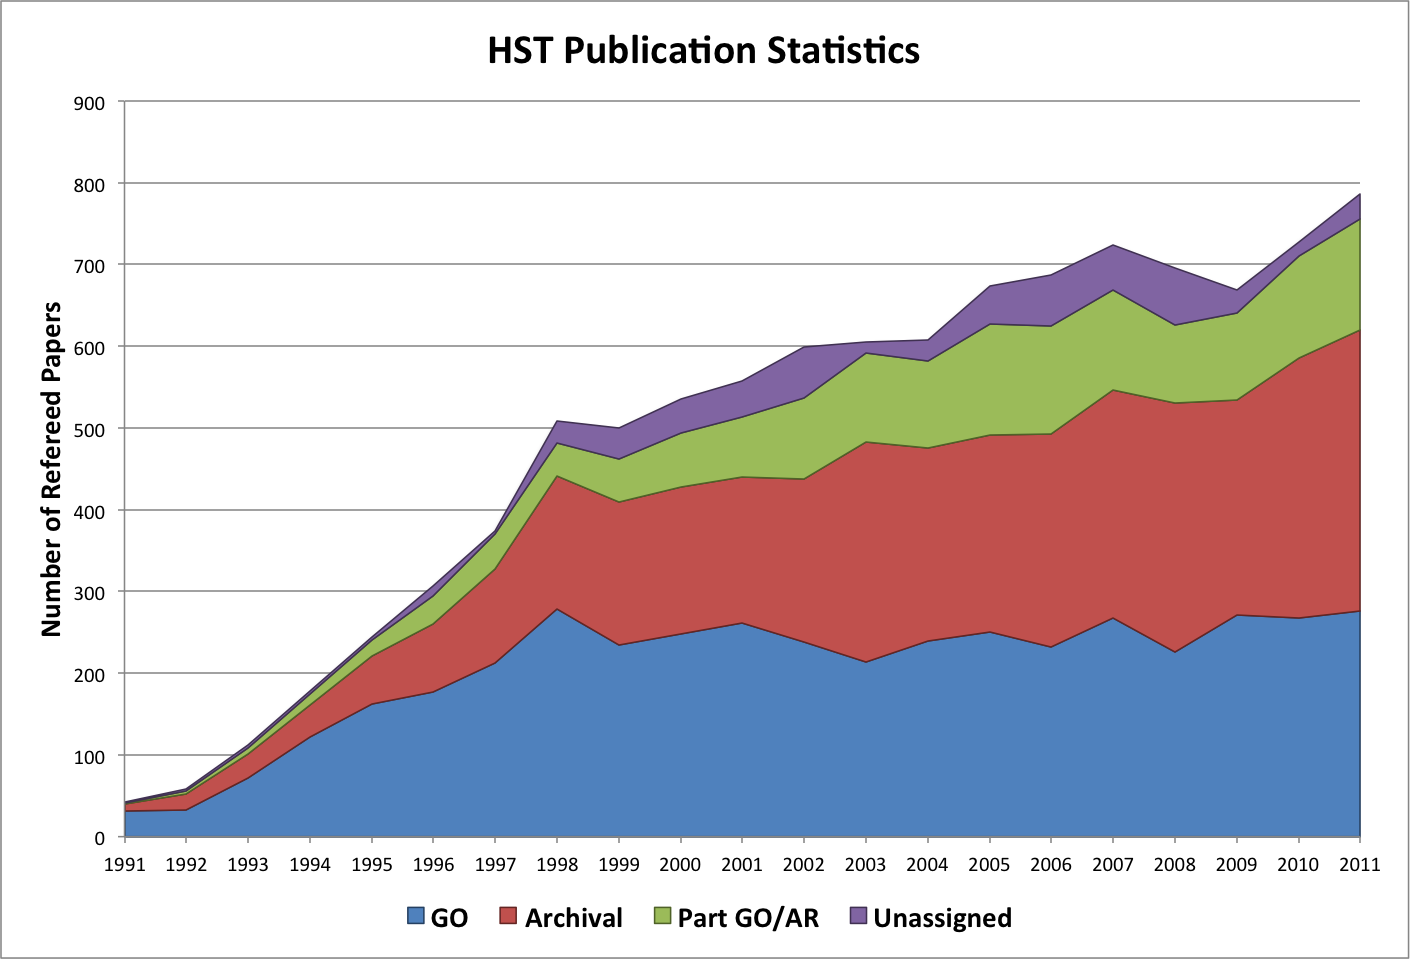
\includegraphics[width=0.75\textwidth]{hstpubs.png}
\hspace{0.03in}
\caption{\small \setlength{\baselineskip}{0.85\baselineskip}
Number of HST GO and archival papers published as a function of year (figure from
White et. al. 2010, ``The High Impact of Astronomical Data Archives'', ASTRO2010 position paper, 
http://archive.stsci.edu/hst/bibliography/pubstat.html
  }
\label{fig:hst}
\end{figure}

\subsection{Technical Approach Overview}

ADMIT would be an add-on software package that interfaces to the CASA software system 
and ALMA archive, implemented both at the server side of the archive and as a 
desktop application with a full GUI. 
The ADMIT core is the infrastructure layer that defines XML structures and 
programmatic pipelines, extracts and organizes scientific metadata from 
image cubes, defines the application programming interface (API) for higher-level tools, 
provides for I/O interaction with the XML, and computes scientifically relevant 
quantities. Built upon the infrastructure layer are specific pipelines to produce 
Basic Data Products (BDP) and the ADMIT Tools that provide advanced functionality 
for scientific analysis. ADMIT is targeted at both a novice user 
(via the convenient GUI), as well as an experienced user (via a Python toolkit 
within the CASA framework), and is designed to be extensible.

The interface to CASA is accomplished primarily through XML files and Python 
scripts. Where possible, ADMIT will call CASA tasks via the XML parameter files 
to accomplish computations. The new tools in the proposal will be Python or 
CASA tasks, depending on the required level of access to CASA data and 
whether the task requires speed optimization through more direct access to the 
CASA core routines. ADMIT will be designed and tested to work in the CASA environment.

\subsubsection{ADMIT Interface to ALMA Archive}

The interface to the ALMA Archive will be simply through the creation of an 
ADMIT data package: a tarball or other standard package format as requested by 
the Archive. The ADMIT data package will be ingested, archived, and served 
to the user as a single item. The user downloads the ADMIT data package by 
selecting it through the standard ALMA Archive interface. This approach has been 
discussed with members of the ALMA archive team (Felix Stoehr and Mark Lacy) and 
is straightforward. Since ADMIT outputs are standard XML and PNG images, 
it is a future option for the Archive Database to ingest the ADMIT information 
to enhance the archive search capability; it is not a baseline requirement for 
ADMIT but it is designed as a feature.

\begin{figure}[t]
\centering
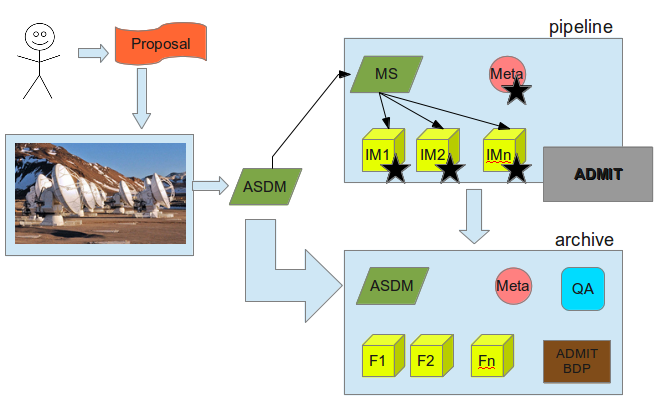
\includegraphics[width=0.75\textwidth]{admit-flow1a.png}
\hspace{0.03in}
\caption{\small \setlength{\baselineskip}{0.85\baselineskip}
ADMIT and ALMA archive interface. Admit is an add-on suite that works
on the data cubes output from the ALMA pipeline and their associated
metadata (all marked with the black star symbol) ADMIT creates the
Basic Data Products that are placed into the archive with the data.
  }
\label{fig:Flow1}
\end{figure}

Figure 2 shows how ADMIT slots into the Reduction Pipeline and ALMA Archive. 
The ADMIT core processes (gray box) are executed after the observatory certifies 
that the image cubes meet proposal science requirements. Information for the BDP 
is gathered from the image cubes, relevant ALMA pipeline metadata outputs, and 
calculated quantities. These are packaged into a file that is ingested (brown box). 

\begin{figure}[t]
\centering
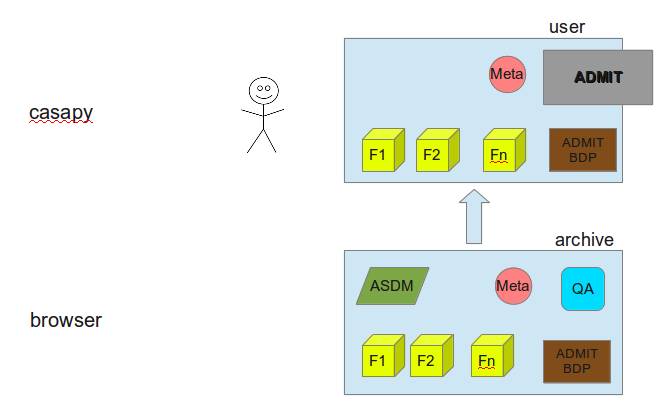
\includegraphics[width=0.75\textwidth]{admit-flow2a.png}
\hspace{0.03in}
\caption{\small \setlength{\baselineskip}{0.85\baselineskip}
ADMIT Basic Data Products in the archive browser (bottom) and downloaded
onto the user desktop. The downloading of the actual data cubes is not 
required to be able to view the BDP; it is required if the user wishes
to recalculate BPP on the local machine.
  }
\label{fig:Flow2}
\end{figure}

Figure 3 shows the ADMIT BDP in the archive. Through the standard ALMA Archive browser 
interface, they can be downloaded to a target machine and viewed either through the 
ADMIT GUI or the Python toolkit interface.

\subsubsection{Infrastructure Layer and Pipeline}

The infrastructure of ADMIT consists of a CASA-compatible Python module of access 
routines and an XML-format metadata file. The XML metadata file, created in the BDP 
or by any re-running of the ADMIT script locally, contains information about the 
observational configuration, source, data statistics, and discovery information about 
the identifications of the lines in the observed bands, channels with detected lines, 
and data products. Simple routines access this metadata to retrieve information as 
needed for the current operation. For interfacing to CASA tasks, the metadata is 
used to construct XML parameter files which are used to run the task. Each ADMIT 
operation builds additional detail into the XML file creating a more 
comprehensive, scientifically useful description.

The ADMIT pipeline is a series of operations that create metadata then 
utilize the metadata to create higher level products.  This approach is simple to 
expand to add further operations or to customize for specific applications.  
The default ADMIT pipeline consists of the summary information, noise levels, 
spectra, line identifications, moment maps, overlap intervals, and image 
saliency information.  ADMIT can work with images in both FITS and CASA format. 
The outputs of the pipeline are wrapped into a single, self-describing tar file, 
which any ADMIT Tool can parse and manipulate. A typical tar file might 
contain a descriptive XML file and associated small FITS and PNG files.

Figure 4 shows a mock-up of the ADMIT initial screen as invoked on the
local user computer. ADMIT next searches the local directory for ADMIT
BDP files and displays a mock-up in Figure 5 indicating what it found and
some instructions. Figure 6 shows a mock-up of how the summary data page
could for a target source in the datasets that ADMIT found. The multiple
tabs along the top are for different sources. The items down each column
show types of data available, spectra, moment zero,
one or two maps, etc, click on the data-cube image puts up a more detailed
page for that item.

ADMIT runs at the ALMA pipeline-archive interface to create the initial BDP, 
but it can also be called by a user from within 
the CASA Python environment as individual commands or a script. This flexibility 
allows a user to tweak the ADMIT settings, add user functionality for a 
specific survey or project, or create more complete metadata.  
The infrastructure can encompass multiple projects and sources, and perform the 
same operations on each source. This can be done either in parallel or recursively. 
It can then extract information from each project and in essence mine a large 
suite of data, allowing linked data techniques to visualize the extracted 
information and provide new insight on what is common or different in the sources.

\begin{figure}[h]
\centering
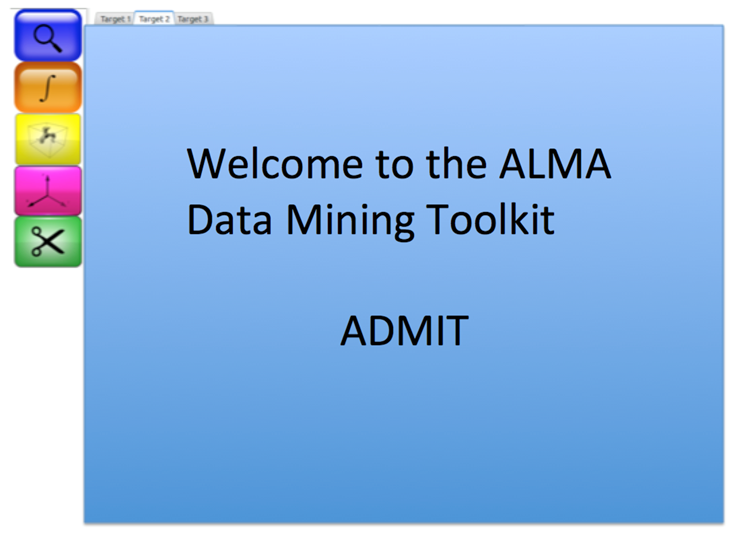
\includegraphics[width=0.65\textwidth]{welcome.png}
\hspace{0.03in}
\caption{\small \setlength{\baselineskip}{0.85\baselineskip}
Mockup of the start screen of the ADMIT GUI (desktop application).
On the left from top to bottom are buttons to invoke ADMIT Tools
(Data Summary, Moment, Feature Extraction, Saliency, and Line Cube Cutout)
for the target source selected in the middle panel. On the top row, tabs
are visible for a number of collected sources.
  }
\label{fig:layout}
\end{figure}

\begin{figure}[t]
\centering
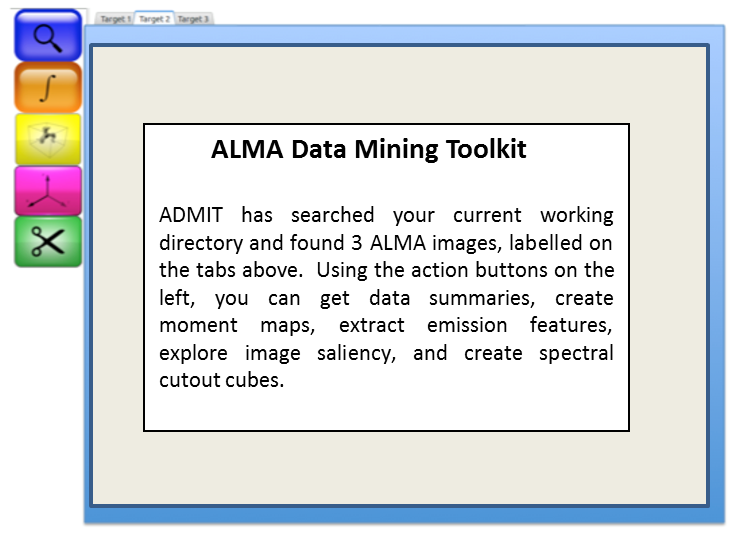
\includegraphics[width=0.65\textwidth]{search.png}
\hspace{0.03in}
\caption{\small \setlength{\baselineskip}{0.85\baselineskip}
Mockup of screen of the ADMIT GUI (desktop application).
ADMIT would automatically scan the local directory for
ADMIT files and load them into the interface if found.
  }
 \label{fig:layout2}
 \end{figure}

\subsubsection{The Toolkit}

Once the core ADMIT components have created the XML metadata, ADMIT uses 
the toolkit component to explore the metadata and make it direct assessable 
the user (both novice and expert).  This is possible because ADMIT defines a 
standard architecture that allows users to use existing analysis tools or to 
create and ``plug in'' their own analysis tools to ADMIT.  ADMIT provides an 
API for these tools to call existing CASA commands, manipulate images or metadata, 
compute new quantities, return data structures to casapy, and store results 
in the tar file with new metadata written to the XML.  Below we described the 
initial set of tools accessed in the GUI that will typically be run as a 
desktop application (see Figure 4).  These tools will deliver science mining 
applicable to a broad range of sources and encapsulate the best methodologies 
arrived at through the community’s many years of experience. 

\subsubsection{Data Summary}

The Data Summary gives the scientist a quick, visual answer to the question: 
``What’s in my data?''  ADMIT answers that question, but as a powerful addition, 
the Data Summary also provides the answer to that question at any point or 
step in the analysis process.  ADMIT collects metadata and writes them to 
an XML file based on a set of ADMIT schema. The metadata are gathered from the 
image cube headers, any metadata produced by the ALMA pipeline, and computed 
quantities from the ADMIT pipeline. When run locally, the default is to gather 
the XML data from all ALMA image files in the current directory. Some components 
of these metadata contain project information (e.g., sources, sky positions, 
ALMA bands used), others may be computed values (e.g., image statistics such as 
min, max, mean, robust median, RMS per channel, etc.), still others will be 
determined by any previous workflow from ADMIT analyzes. Each ADMIT Tool 
operation will update the metadata so that an up-to-date summary of everything 
that has been gathered and computed is quickly presented (Figure 6).  
Selecting a particular band, line, or source would open up more detailed 
views of the BDP.

\begin{figure}[t]
\centering
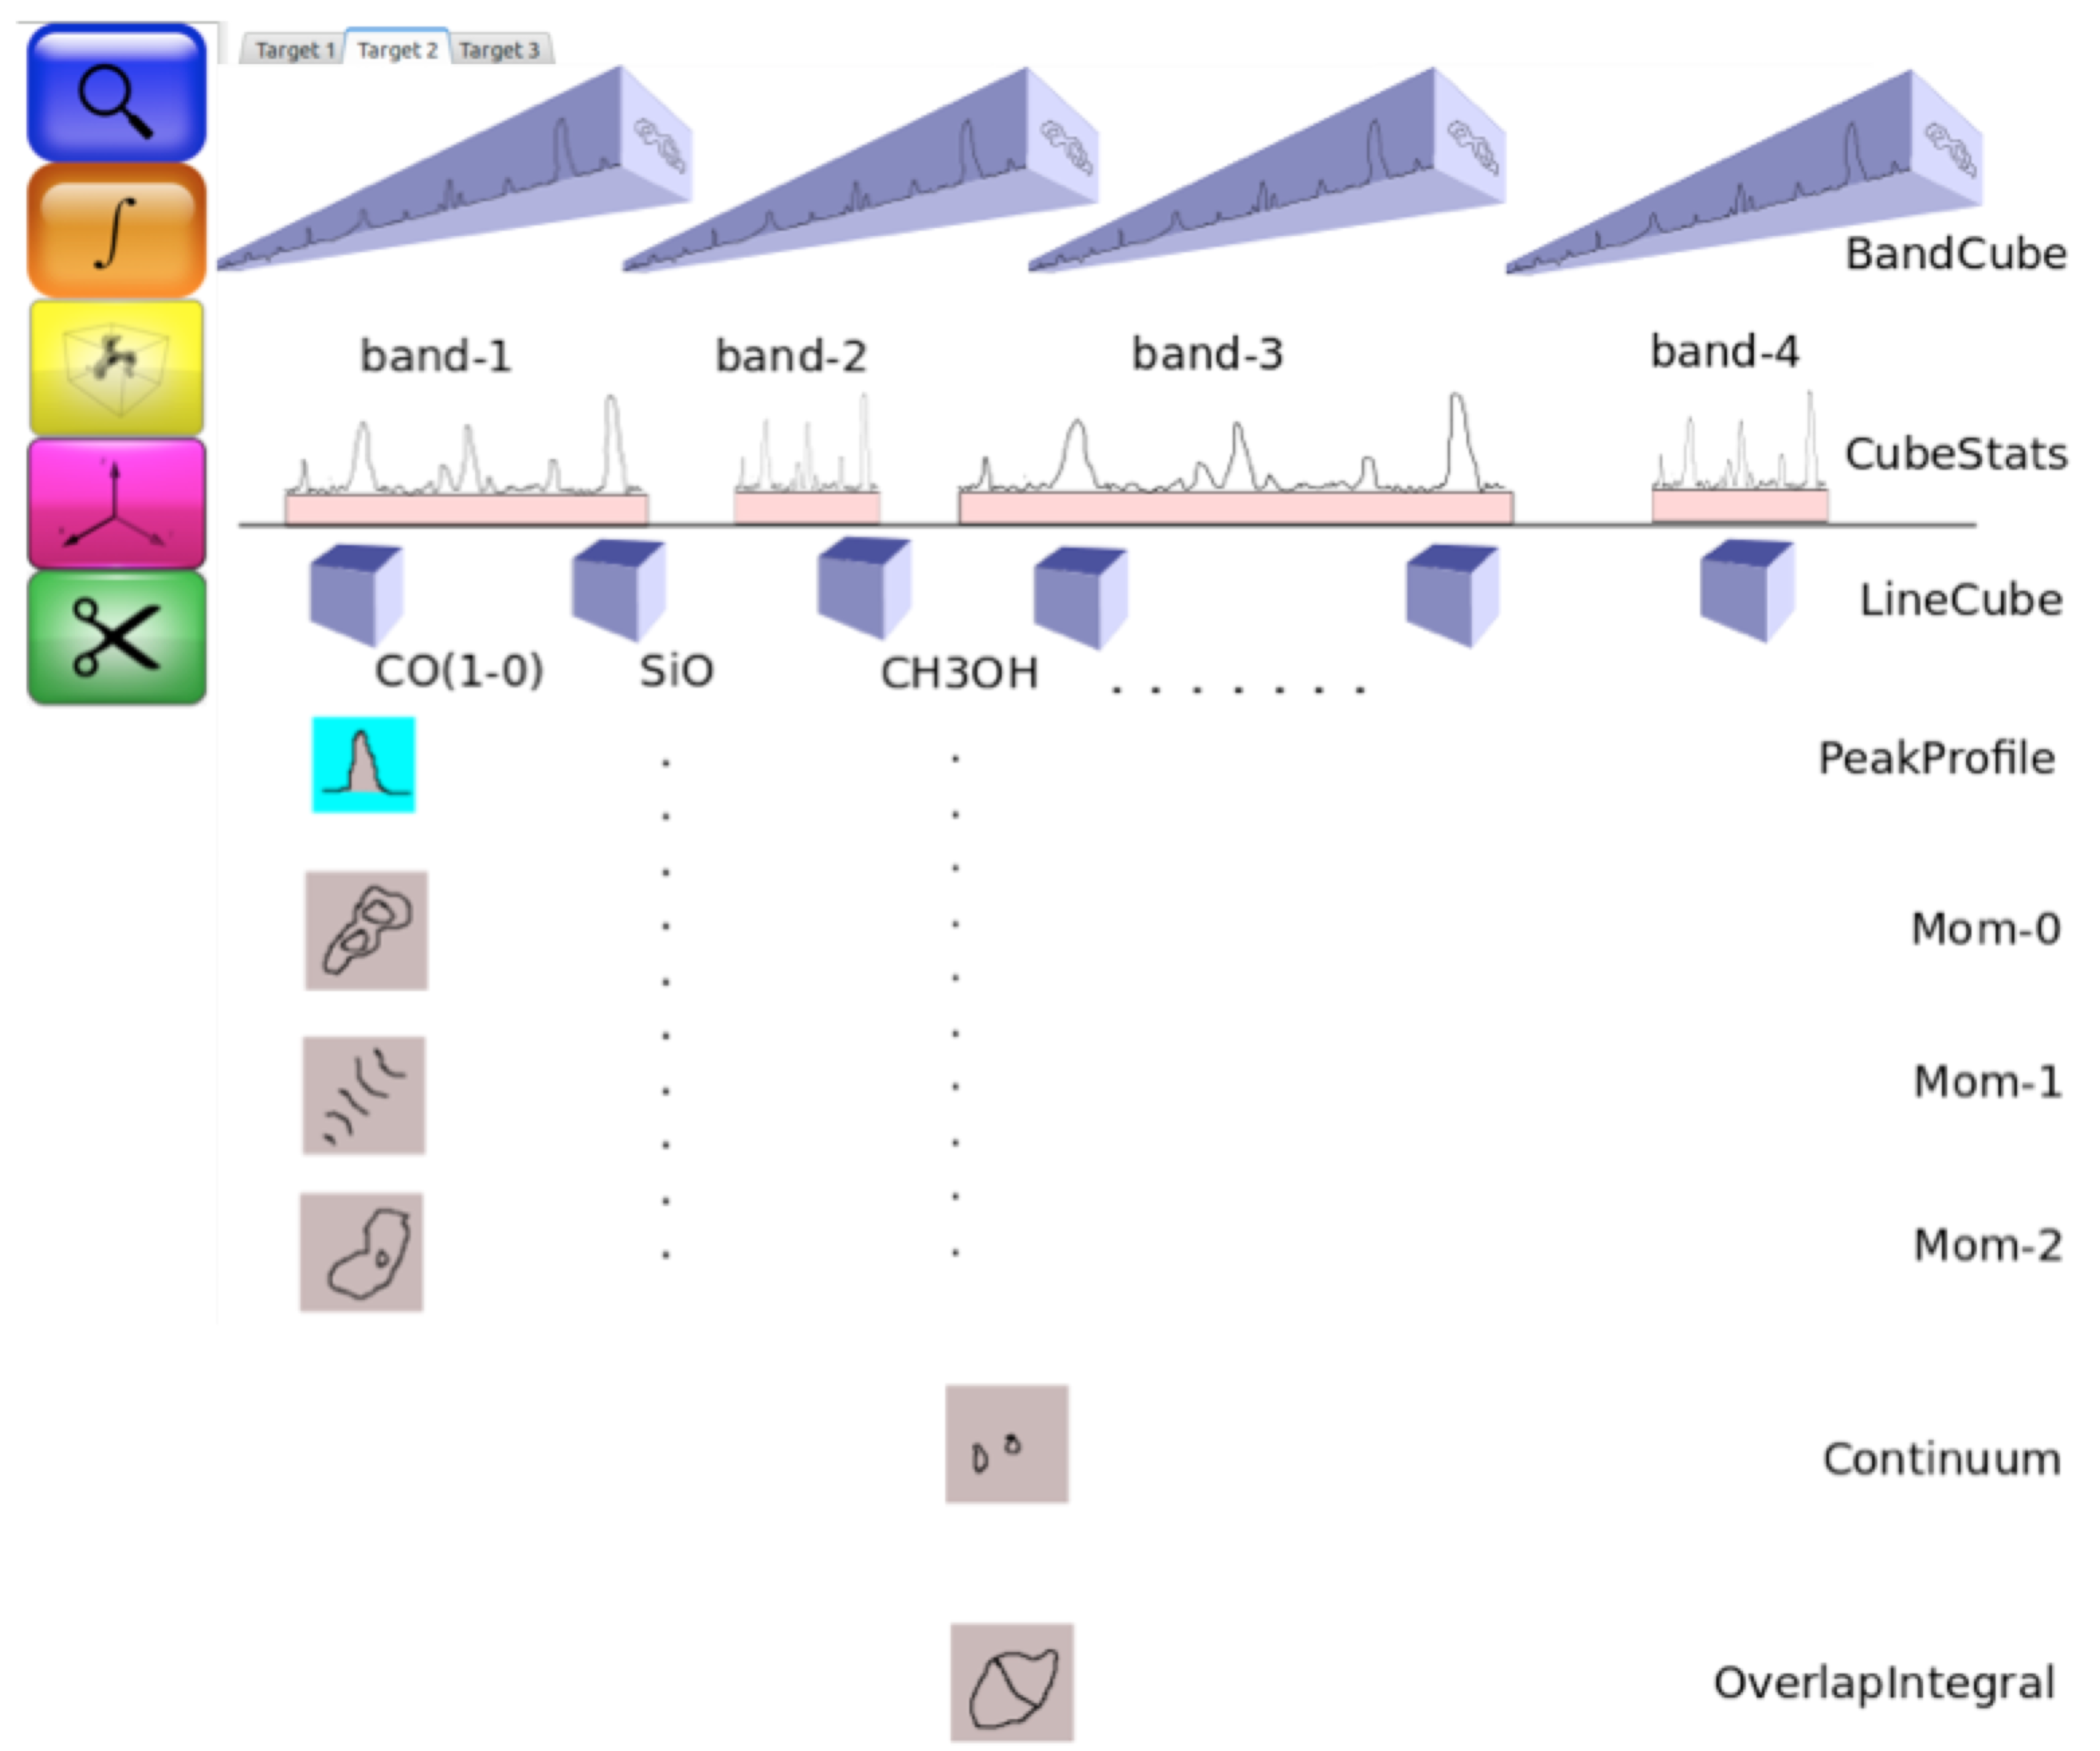
\includegraphics[width=0.85\textwidth]{overview.png}
\hspace{0.03in}
\caption{\small \setlength{\baselineskip}{0.85\baselineskip}
Mock-up of screen of the ADMIT GUI (desktop application).
The data summary page give the user an overview of the data there were
present for a given source. Each row show the output of an ADMIT tool
operation listed on the right, giving an easy-to-understand visual summary
of the science data and tool outputs for the target source selected in the
middle panel. On the top row, tabs are visible for the collected sources.
  }
\label{fig:overview}
\end{figure}

\subsubsection{Example Use Case}

In this use case scenario, the user has already downloaded a number of projects from the ALMA archive, and all have the basic ADMIT data included. The hypothesis to be checked is if the line width in CO correlates with the presence of a selected number of molecular lines, in the sense that for wider profiles some of the molecules would be destroyed, and thus the overlap integral would not achieve the maximum value (where all molecules are present).  In this case the user selected CO as the reference line, and C17O, CS, and H13CN as probes. In this example the user is more interested in a global value per object, than a point by point comparison in the map.

The code loops over all projects, and first ensures that all lines are represented. It estimates the line width from the PeakProfile (precomputed by ADMIT) in the CO line cube as a representative value for the line width for the object.  This particular user is conservative and wants to recompute the integrated flux (moment 0) maps with a 3-sigma clip. These new moment maps are then turned into an overlap map (one of the ADMIT tools) and via some simple NumPy math the fraction is computed from number of pixels with value 15 (where all lines are present) divided by the number of pixels with any signal in any of the lines (overlap map value more than 0).  The line width is then plotted against this fraction, with the expectation that it starts near 1 and then suddenly drops at some line width.   In the example code is shown below, one can see the power of ADMIT:  in just a few lines of simple Python, a scientific hypothesis can be created and examined based on ALMA images.

\begin{verbatim}

import admin, math                             # grab some needed python modules
import numpy as np                             #

adm = admit.ADMIT()                            # initialize ADMIT

projects = adm.query_dir('.')                  # look for ADMIT projects here

lines = ['co', 'c17o', 'cs', 'h13cn']          # first line is reference line
omax = math.pow(2,len(lines))-1                # max in overlap map, 15 in this case

s_list = []                                    # accumulate line widths
f_list = []                                    # accumulate fractions

for p in projects:
  adm.setdir(p.dirname)                        # move into the proper project directory
  line_cubes = {}
  for c in p.linecubes:                        # loop over line cubes and grab the line name
    if lines.count(c.line):                    # if we got one of the lines we wanted
       line_cubes[c.line] = c                  # store reference to that line cube

    if len(lines) != len(line_cubes):
       print "Skipping ",p.dirname
    continue

  c_ref   = line_cubes[lines[0]]               # reference to the CO cube
  x       = c_ref.peakprofile('vlsr')          # spectrum X in KM/S
  y       = c_ref.peakprofile('value')         # spectrum Y in JY/BEAM
  x_mean  = (x*y).sum()/y.sum()
  x_width = (x*x*y).sum()/y.sum() - x_mean*x_mean 

  s_list.append(x_width)                       # accumulate for later

  m = []                                       # accumulate maps for new overlap
  for l in lines:                           
    m0 = adm.moment(c,[0],'clip',rms=3*c.rms)  # compute new moment maps
    m.append(m0)

  o = adm.overlap(p,m)                         # get overlap image
  oval = o.array()                             # get a numpy reference for work
  f_all = len(np.where(oval == omax)[0])       
  f_sig = len(np.where(over > 0)[0])

  f_list.append(f_all/f_sig)
  #
#
adm.plot2d(s_list,f_list)                      # scatterplot of accumulated data 
							        
\end{verbatim}


\section{ADMIT Tools}

This section shows some of the tools that we have
been prototyping for ADMIT. The tool are layered on top
of the XML infrastructure of ADMIT and  communicate through
that sturcture for inputs and outputs. We envision
that there will be a set of basic tools that create some
of the Basic Data Products and there will be an evolving
set of tool that add new capability. The tools will be
compatable with the CASA environment and utilize the CASA
core and existing CASA routines where applicable. The tools
will operate on CASA image format data.

A second operational goal for tools is that they can
be re-executed based on data in the ADMIT XML files and the
XML files can be modified to allow the tools to be re-run
in bulk. For example, if you decide to change the velocity
range for a moment map, you could modify the XML information
and then re-run the moments for all of the lines of interest with
with a single command.

\subsection{Line Identification and Line Cutout}

The Line ID Tool will compare the rest frequency coverage of the 
image cubes with a database of common line retrieved from Splatalogue to 
identify the appropriate channel/cube locations of potential lines.  
A line-strength vs. frequency table is the essential input into a line 
identification procedure (here we will leverage Tony Remijan’s datasplat project). 
The input data for the procedure will be improved by the previously computed 
per-channel cube statistics and aided by cross-correlation techniques in a 
position-velocity diagram (Figure 7) or in the cube itself. The output will 
be a series of identified and unidentified lines across the different bands 
in a simple table of line, frequency, channel range, and detection probability.

\begin{figure}[t]
\centering
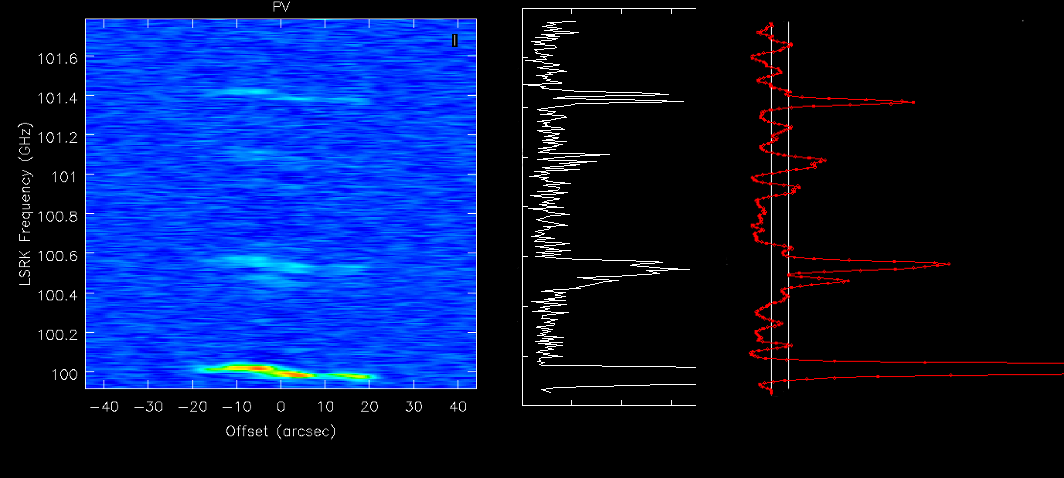
\includegraphics[width=0.75\textwidth]{line-id.png}
\hspace{0.03in}
\caption{\small \setlength{\baselineskip}{0.85\baselineskip}
Line identification can be tremendously improved in a position-velocity diagram
by cross-correlating the signal in the velocity direction. In Figure 7, compare the more
traditional noisy peak/RMS plot in the middle (white) with the smooth
cross correlation technique on the right (in red). The lines are better
resolved using the cross-correlation technique. The two vertical lines
denote zero (white line) and a 3-sigma clipping (gray line).
  }
  \label{fig:hst}
  \end{figure}


Based on the line identification line tables, line cutout cubes can be 
extracted, with now the third axis in Doppler velocity space, to ensure that 
we can compare the different lines and molecules on the same basis. Depending 
on the number of lines in the bands, keeping only the line cubes can significantly 
cut down user disk usage.

\subsection{Moment Maps}

Moment maps are a simple, yet powerful tool for examining global properties 
of an object’s emission. The most commonly used maps are integrated flux 
(moment 0), centroid velocity (moment 1), and velocity dispersion (moment 2).  
The Moment Map tool takes the line cubes produced by the Line ID Tool and 
creates the three moment maps for each spectral line (see Figure 8). The moment 
can be clipped based on simple RMS cutoff (already computed by the Data 
Summary tool!), but also could employ more sophisticated methods such as local 
smoothing to increase the signal to noise to create a more robust clipping mask. 
Moment maps can also be produced using parametric shapes, e.g. a Gaussian fit, 
which would then store the total emission, mean velocity and width of the 
spectrum at each location.

The advantage of the ADMIT approach is that the previous steps of line definition
and rest frequency assignment allow automated calculation of the velocity scale
for each line. This can be combined with simple spectra at peak position as
shown in the mock-up figure.

\begin{figure}[t]
\centering
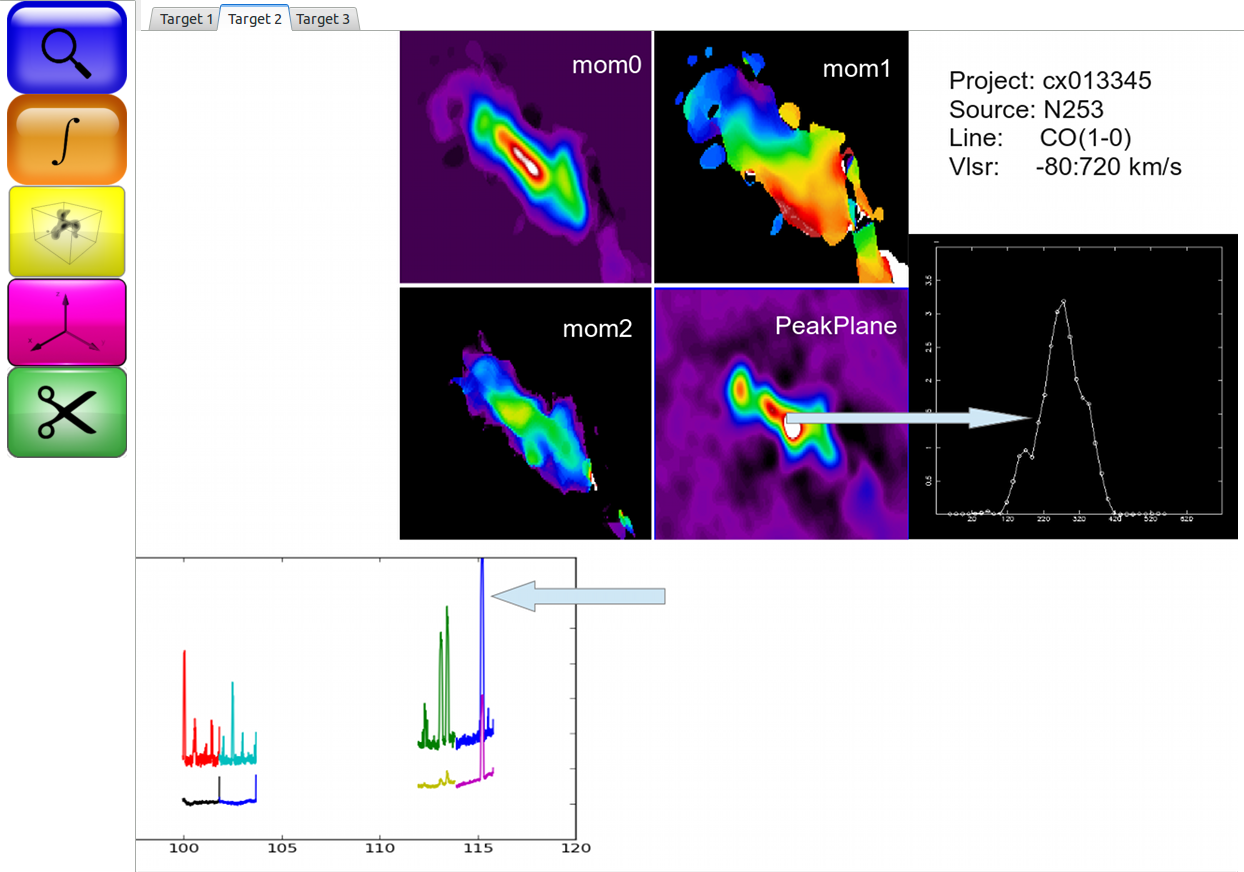
\includegraphics[width=0.75\textwidth]{moments.png}
\hspace{0.03in}
\caption{\small \setlength{\baselineskip}{0.85\baselineskip}
Mockup of the detailed view of some of the data products of a 
single source and spectral line, as produced by the Data Summary tool \
for the target source selected in the middle panel. In this scenario, 
the user has clicked on the CO data cube icon in Figure 6. 
On the top row, tabs are visible for a number of collected sources. 
The lower arrow indicates which line is the CO line in the full-band 
spectra. The upper arrow indicates the reference position for the spectrum shown.
  }
 \label{fig:moments}
\end{figure}
 

\section{Exploration of New Algorithms}

To enable the creation of an interactive analysis, 
reasoning, and discovery environment, new methodologies are needed to
detect and effectively presentation the scientifically interesting data
buried in large ALMA data cubes.
The fundamental fact is that most of the pixels in any data cube are noise,
and data cubes with significant signal density (many lines and/or many spatial
features) are difficult to mine for science content. 

Much of the science with large data cubes to date has been accomplished with
simple information compression techniques: moment maps, velocity position
diagram along selected axes, rotation curve fitting, and visual inspection
for eye-catching correlations. Analysis such as principle component 
analysis and other orthogonal component decomposition analysis have been
applied for analyzing structure in complex environments such as molecular
cloud. In general, however, the generally available techniques in standard
radio astronomy data reduction packages have not change in major ways in
over 20 years.

As a part of this study, we have looked at the kinds of new analysis tools
will be of high value to astronomy for: (1) comparing the characteristic
of emission within a given line at different velocities, in  different lines,
for the same line in different sources. The subsections below discuss two
specific examples that we explored at the level of creating prototype tools.

\subsection{Overlap Integral}

The overlap integral provides an overview of the emission properties across
a number of spectral lines; it can also be generalized to apply
to the emission as a function of velocity within a line or across source. 
In the multi-line application,
for each detected line, one assigns a one or zero indicating the presence of emission
at some selected level, and
then logically ORs them across all lines, creating a bit-mask map of the emission
present in each spatial-velocity pixel. One can do this in a moment map, or a cube, to determine in
which spatial or velocity regions certain lines are present or absent in relation to
other lines. 

The final image or cube is a integer map with 0/1 in each bit representing the presence/lack
of emission in one of the lines. This integer is then easily displayed as a color image.
An example using NGC 253 spectral line data from ALMA Cycle 0 is
shown in Figure 9. This technique can also be applied to individual channels of
a single spectral line to examine the velocity pattern of emission, similar to a renzogram.

\begin{figure}[t]
\centering
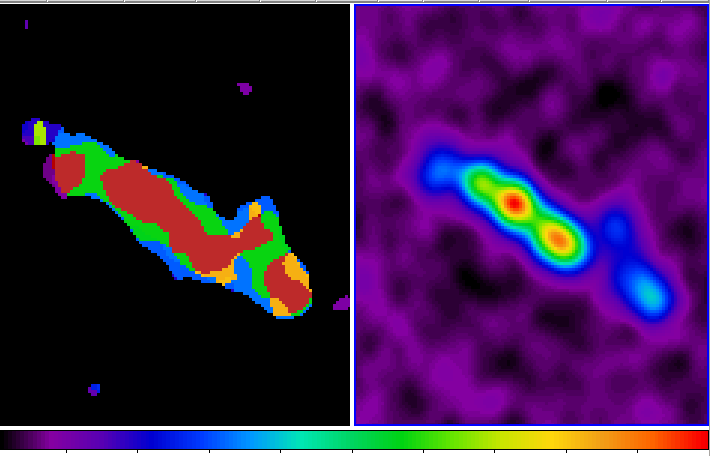
\includegraphics[width=0.75\textwidth]{overlap.png}
\hspace{0.03in}
\caption{\small \setlength{\baselineskip}{0.85\baselineskip}
An example of an overlap integral using ALMA Cycle 0 data of NGC~253. Right: Integrated flux
(moment zero) image of the CO J=1-0 emission. Left: The combined overlap integral -- valued from
0 to 255 -- of 8 spectral lines. Each line is represented by a single bit in an 8-bit
integer which is then translated into a color scale. As can be seen, most of the peaks
have all 8 lines present (red). The spectral lines used to create this overlap integral are
CO, C$^{17}$O J=1-0, CN J=1-0 F=1, CN J=1-0 F=2, HC$_{3}$N, CH$_{3}$OH, H$_2$CS,
and CH$_{3}$C$_{2}$H.
  }
\label{fig:hst}
\end{figure}

\subsection{Descriptor Vectors}

One technique from computer science with significant potential for implementation
in astronomy is "descriptor vectors". The approach is to segment an image or
cube and and calculate an n-dimensional description vector to characterize each
segment. One of the current applications of this technique in visual image analysis
is in automated feature identification. In this application, the image is segmented
into M-regions and each region is characterized by an n-dimensional vector which
might simply the intensity distribution of the pixels within the segment, or the
pixel color distribution, or contrast level; it could be that the segment is characterized
by the spatial shape distribution. Once the vectors are generated, then it is
easy to calculate the "distance" between the various vectors and to identify
which vectors are most like, or unlike, each other. One can identify clusters
of vectors. This gives you an ordered list of locations in the image or cube
that share similar characteristics.

The descriptor vector approach
provides an application-independent, purely mathematical measurement of information 
(M. Chen and H. Janicke. ``An information-theoretic framework for visualization''
IEEE Transactions on Visualization and Computer Graphics, 16(6):1206 –1215, 2010;
H. Janicke and M. Chen. ``A salience-based quality metric for visualization''
Computer Graphics Forum, 29(3):1183–1192, 2010).  
For astronomical images, description vectors can be chosen from any number of 
properties of the emission.  An example in vision research utilizes a color 
histogram, which enables a very fast cataloging of feature types in an image, 
as well as finding the features similar to a selected one, a type of machine learning 
(C. Y. Ip and A. Varshney, ``Saliency-assisted navigation of very large landscape 
images'', IEEE Transactions on Visualization and Computer Graphics, 17(12):1737– 1746, 2011;
C.Y. Ip, Ph.D. Thesis, University of Maryland, 2014).
We have imported several astronomical data cubed into existing descriptor vector
software associated with the work by Mr. Ip (UMD computer science graduate student)
and Professor Amitabh Varshney (UMD Professor in computer science).  One of the
aspects of the descriptor vector method is that you have a set mechanism for
how to proceed but you have wide latitude in how you segment the image and the
mathematical prescription for calculating the n-dimensional vector. This makes
the method very versatile.

It is important to note that
although this may sound similar to Principal Component Analysis, the descriptive 
vectors do not need to be orthogonal or even have the same units. Because of the
versatility and the specific focus possible with tuned vector formulations,
data mining with this technique can be an extremely powerful, allowing a 
fast comparison of features that might be missed otherwise.  

During our study, we evaluated this technique’s 
potential for achieving astronomical science goals.  The key to success is discovering the best 
description vector for the specific science case (M. Chen and H. Janicke. ``An 
information-theoretic framework for visualization'', IEEE Transactions on Visualization 
and Computer Graphics, 16(6):1206 –1215, 2010).   For example, in one case 
the descriptive vector that best describes a specific science goal may be the properties 
of the certain molecular lines and the overlap interval, while another may be the 
location of the molecular peaks with respect to the continuum.  ADMIT can provide the 
infrastructure to write various descriptor vectors, provide some of the vectors 
(based on BDPs) that will most likely to cover standard science goals, and provide a 
task that determines best vector choices based on user inputs.   
We will also document the descriptor formulation procedure so that users have the 
option to build on this approach in the future.   

There are, of course, no significant barriers to generalizing this approach to
comparing multiple lines or multiple sources. For example to be able to ask questions
like: Where in my data cubes to HCN and CO have overlapping emission but there
is no HNC emission? Give me a list of all of the position-position-velocity locations
were SO and SiO emission are coming from the same locations. Or, give me a list
of the places where the CO is falling off rapidly with velocity and there is
SO emission.

\subsection{Learning Algorithms}

In computer science applications, the descriptor vector characterization of an image
can be layered with learning algorithms which can power efficient data mining. The
simplest application is to make a descriptor vector description of an image or
cube then to manual look at the image or cube and identity a region of interest.
The algorithm can then calculate which other segments have similar vectors to your
selected regions, providing an ordered list of the 10 nearest vectors. One can
then view those regions, select which ones are correctly of interest; feed the
new set of regions if interest into the algorithm and get a new ordered list of
most similar vectors/regions. 

This combination of compact description approach and learning-selection is very
well suited for combination with a visualization tool. The algorithms here 
provide a computing layer which provide an order list of interested regions in the
cube for display in the visualization tool. The visualization give the user
rapid feedback to refine the search; the list of preferred regions is feed back
into the algorithm for an increasingly targeted search.


\section{Intercomparison of Model and Observational Data}

As the study progressed, we felt that this area was of less
importance than continuing to development the XML structure
design for ADMIT. By adopting the CASA and its python environment,
we will be able to adopt python based program for reading output
from modeling programs and simulations into a common format.
During the course of our study, we also learned that CASA was
in the process of evaluating its approach to the python environment.
Changes there could make a wider range of existing programs
easily available for use.


\end{document}

%%% Local Variables: 
%%% mode: latex
%%% TeX-master: t
%%% End: 
